% ARR / EMNLP long-paper submission (review mode, anonymous).
% Build: pdflatex main && bibtex main && pdflatex main && pdflatex main
\documentclass[11pt]{article}
\usepackage[review]{acl}

\usepackage{times}
\usepackage{latexsym}
\usepackage[T1]{fontenc}
\usepackage[utf8]{inputenc}
\usepackage{microtype}
\usepackage{inconsolata}
\usepackage{graphicx}
\usepackage{booktabs}
\usepackage{multirow}
\usepackage{xcolor}
\usepackage{amsmath}
\usepackage{amssymb}
\usepackage{enumitem}
\usepackage{fancyvrb}
\usepackage{placeins}
\usepackage{tikz}
\usetikzlibrary{arrows.meta,positioning,calc,decorations.pathreplacing}
% MemoHarness / SkillRC figure palette
\definecolor{phaseA}{HTML}{6F9AD3}
\definecolor{phaseB}{HTML}{B07A8F}
\definecolor{gptblue}{HTML}{5F86C2}
\definecolor{qwenmint}{HTML}{4FA58C}
\definecolor{salmon}{HTML}{D9735A}
\definecolor{sand}{HTML}{B8923A}
\definecolor{contractv}{HTML}{6B4C9A}

% Shared notation and macros.
% \pending{...}: a number that is not available yet (run still in progress). Every use must be
% replaced by a value from paper/data/results.json before submission.
\newcommand{\pending}[1][]{\textcolor{red}{\textbf{[pending#1]}}}
\newcommand{\figplaceholder}[2]{%
  \IfFileExists{#1}{\includegraphics[width=\linewidth]{#1}}{%
    \fbox{\parbox[c][#2][c]{0.95\linewidth}{\centering\small\textcolor{gray}{figure in preparation: \texttt{\detokenize{#1}}}}}}}

% Arms (names follow Zhang et al., 2026: ActionSFT / ActObs)
\newcommand{\armA}{ActionSFT}
\newcommand{\armB}{ActObs}
\newcommand{\armC}{ActionSFT-LR}
\newcommand{\armD}{ActionSFT+Wiki}
\newcommand{\armE}{Outcome-Aux}
\newcommand{\armF}{Outcome-in-Action}
\newcommand{\armG}{Contract}
\newcommand{\armGp}{Contract-Placebo}

\newcommand{\KL}{\mathrm{KL}}
\newcommand{\CE}{\mathrm{CE}}
\newcommand{\passat}[1]{pass@#1}

% Upstream report of the empty-gold reward. Empty in the anonymous review build; the public build
% (site/build_assets.sh) defines it as the issue number before this file is read.
\providecommand{\skyrlissue}{}


\title{Know2Act: What Knowledge Reaches\\a Tool-Using Agent's Actions?}

\author{Anonymous ARR Submission}

\begin{document}
\maketitle

\begin{abstract}
Recent work trains language agents to predict not only their own actions but also the observations that the environment returns, and reports that this makes later reinforcement learning (RL) more effective because the agent learns the consequences of its actions. We ask whether knowledge learned in this way reaches the agent's decisions. In Know2Act, a pre-registered study of a multi-turn text-to-SQL agent trained with supervised fine-tuning and then GRPO, we measure what each model learns and how it acts. Observation supervision is learned: on unseen databases the agent predicts the format and headers of result tables far better. Yet it changes the agent's actions less than reshuffling the training data does, and it brings no gain after RL. We then vary what the agent predicts and where, up to a contract that states the shape of the correct answer and is checked against every query result. Every prediction is learned, but none changes when the agent submits an answer or keeps querying. The knowledge is usable from outside: selecting among sampled answers with the agent's own contract improves accuracy. RL, which rewards only the final answer, removes even this gain and makes the agent more willing to submit after its own check has failed. Learning to predict the environment is therefore not the same as acting on the prediction. We also find that 44\% of the training tasks in a public SQL RL environment reward an empty answer.

\end{abstract}

\section{Introduction}
\label{sec:intro}

Language-model agents are often trained to say what they expect before they act. ReAct-style thoughts, belief states and plans all put a prediction in writing \citep{yao2023react,wang2026evu,zhang2025earlyexperience}. Monitors read these predictions to judge why an agent acts \citep{korbak2025monitorability}, and editing them is a cheap way to steer an agent. Both practices assume the written prediction takes part in the decision.

Work on chain-of-thought faithfulness shows that whether this assumption holds depends on the test. Deleting reasoning often leaves answers unchanged, while editing it can change them \citep{lanham2023faithfulness}. In fine-tuned agents, replacing the whole reasoning trace moves fewer actions as training goes on \citep{liu2026cotgains}.

For knowledge that the model has learned, the question is harder. In ordinary training data the written prediction and the knowledge in the weights rarely conflict, so the data do not show which of the two the action follows when they do.

We study the question in a setting built so that the two can be told apart. \alfcf{} is a counterfactual version of ALFWorld in which each object class is kept in a fixed, arbitrary receptacle class, chosen so that neither the original data nor the base model's prior points to it. The location can therefore only be learned from fine-tuning.

At the first search step of an episode, the agent has not yet seen the target, so its one-line prediction, which we call the \emph{note}, is the only location information in its context (Figure~\ref{fig:overview}). We fine-tune Qwen3-4B on six versions of the training data. They differ in one respect each: whether predictions are always followed by the action, sometimes contradicted by it, or followed by an action that ignores them.

At the first search step we then either delete the agent's prediction or replace it with the prediction the agent writes for another object, and record where the agent goes. Each arm is compared with what a perfect imitator of its training data would do, so effects that follow from the data construction are not read as properties of the model.

% Conceptual overview (no bookkeeping numbers). Included from the introduction.
\begin{figure*}[t]
\centering
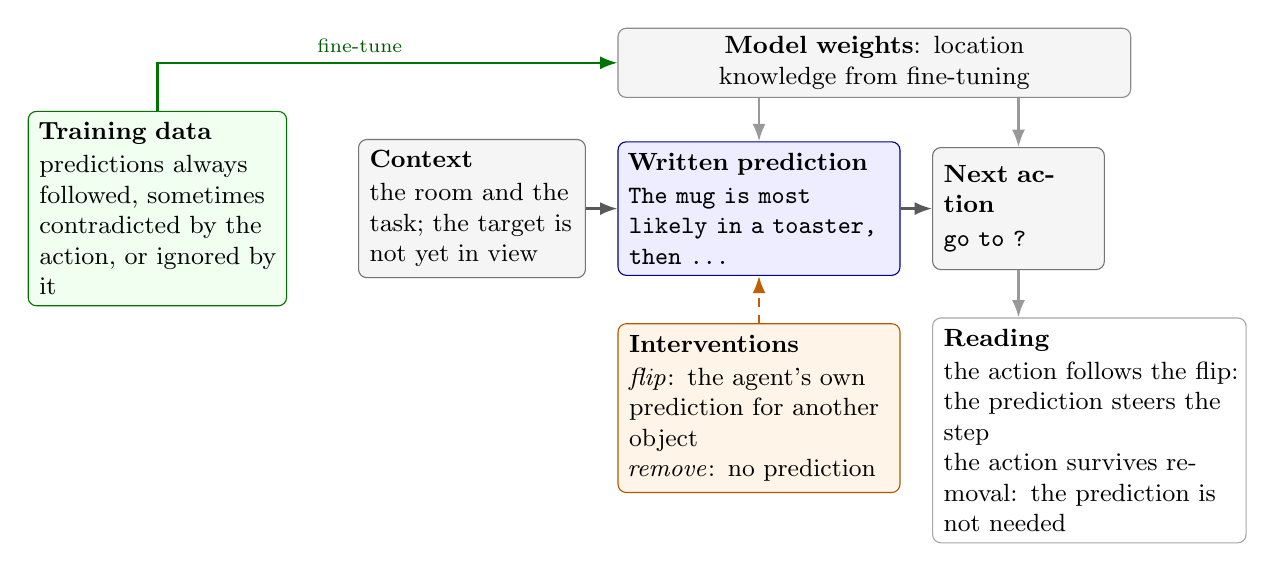
\begin{tikzpicture}[
  font=\small,
  box/.style={draw=black!55, rounded corners=3pt, align=left, inner sep=4pt, fill=white, minimum height=1.55cm},
  ctx/.style={box, fill=black!4},
  note/.style={box, fill=blue!7, draw=blue!55!black},
  act/.style={box, fill=black!4},
  wts/.style={draw=black!45, rounded corners=3pt, align=center, inner sep=3pt, fill=black!4, minimum height=0.6cm},
  ivn/.style={box, fill=orange!9, draw=orange!70!black, minimum height=1.3cm},
  read/.style={box, fill=white, draw=black!35, minimum height=1.3cm},
  data/.style={box, fill=green!6, draw=green!45!black},
  arr/.style={-{Latex[length=2.2mm]}, thick, black!65},
  darr/.style={-{Latex[length=2.2mm]}, thick, dashed, orange!75!black},
]
\node[data, text width=3.0cm] (data) {\textbf{Training data}\\[1pt] predictions always followed, sometimes contradicted by the action, or ignored by it};
\node[ctx, right=0.9cm of data, text width=2.6cm] (ctx) {\textbf{Context}\\[1pt] the room and the task; the target is not yet in view};
\node[note, right=0.4cm of ctx, text width=3.3cm] (note) {\textbf{Written prediction}\\[1pt] \texttt{The mug is most likely in a toaster, then \dots}};
\node[act, right=0.4cm of note, text width=1.9cm] (act) {\textbf{Next action}\\[1pt] \texttt{go to ?}};
\node[wts, above=0.55cm of note.north west, anchor=south west, text width=6.3cm] (wts) {\textbf{Model weights}: location knowledge from fine-tuning};
\draw[arr, green!45!black] (data.north) |- node[pos=0.72, above, font=\scriptsize, green!35!black] {fine-tune} (wts.west);
\draw[arr] (ctx) -- (note);
\draw[arr] (note) -- (act);
\draw[arr, black!40] (wts.south -| note.north) -- (note.north);
\draw[arr, black!40] (wts.south -| act.north) -- (act.north);
\node[ivn, below=0.6cm of note, text width=3.3cm] (ivn) {\textbf{Interventions}\\[1pt] \emph{flip}: the agent's own prediction for another object\\ \emph{remove}: no prediction};
\draw[darr] (ivn) -- (note);
\node[read, below=0.6cm of act.south west, anchor=north west, text width=3.7cm] (read) {\textbf{Reading}\\[1pt] the action follows the flip: the prediction steers the step\\ the action survives removal: the prediction is not needed};
\draw[arr, black!40] (act.south) -- (act.south |- read.north);
\end{tikzpicture}
\caption{The question and the design. Before each search step the agent writes where it expects the target. Fine-tuning puts the location knowledge into the weights, from which it can reach the action directly or through the written prediction. We fine-tune on data that differ only in how predictions and actions are coupled. At the first search step, where the prediction is the only location information in context, we flip or remove the prediction and record where the agent goes. Each training arm is also compared with what a perfect imitator of its data would do.}
\label{fig:overview}
\end{figure*}


When every prediction in the training data is followed, the prediction steers the agent without being needed. Deleting the prediction lowers the probability of the predicted move by 0.015. Replacing it redirects 80\% of first moves across eight seeds, and a randomly ordered ranking, a form never seen in training, is followed even more readily (0.90). In held-out rooms, whether the weights hold a convention for the object makes no detectable difference.

Over a whole episode, writing another object's prediction at every step raises the number of receptacles visited from about two to about nine. The control is strongest at the first step and much weaker later, where it depends on what the search has already shown. Removing the agent's earlier predictions from its history partly restores the control.

When a quarter or half of the training predictions are contradicted by the teacher's action, the agents keep writing predictions but follow a replaced one in at most about 1\% of first steps, within 0.012 of what a perfect imitator of such data does. When half of the actions ignore correct predictions instead, redirection drops to 27\%, between what an imitator would show if it credited its correct actions to the weights (0) and to the predictions (0.50).

For monitoring, this means that when the training data also teach the agent to act without a prediction, as ours do at 30\% of steps, a deletion test calls the predictions decorative, while an edit test shows that they steer the first decision. For training, contradicting a quarter of the predictions was enough to remove that steering.

\section{Observation Supervision, Its Alternatives, and Where Predictions Go}
\label{sec:method}

Every agent trajectory pairs what the agent did with what the environment returned. All the arms below train on the same trajectories in the same order with the same hyper-parameters. They differ only in which tokens carry loss, or in a short line inserted into the text.

\paragraph{Objective.}
Let a trajectory be $\tau=(x,a_1,o_1,\dots,a_T,o_T)$, with task prompt $x$, agent turns $a_t$, and observations $o_t$. Here each $o_t$ is an SQL result table or error message. Let $A$ and $O$ index the action and observation tokens. Following \citet{zhang2026actobs}, we minimise
\begin{equation}
\mathcal{L}_\lambda = -\frac{S_A + \lambda S_O}{|A|+\lambda|O|},\quad
S_X=\sum_{i\in X}\log p_\theta(y_i\mid y_{<i}).
\label{eq:actobs}
\end{equation}
$\lambda=0$ gives \armA{}, and $\lambda=1$ gives \armB{}.

\paragraph{Two readings of a gain.}
If \armB{} helps RL, there are two ways to explain it. On the world-model reading, predicting $o_t$ requires modelling what $a_t$ does, and that knowledge shapes later actions. On the dilution reading, Eq.~(\ref{eq:actobs}) shrinks the action term's share of each update to $|A|/(|A|+|O|)$, which is 0.69 in our data, and fitting actions less could by itself preserve plasticity for RL \citep{plasticity2026}. We pre-registered two controls that reproduce the dilution without any environment prediction. \armC{} is action-only SFT whose learning rate is chosen so that its held-out action KL to the base model matches \armB's; a frozen rule selected $0.85\times$. \armD{} replaces the observation term with the same number of unrelated Wikipedia tokens.

\paragraph{Where the prediction goes.}
Unmasking observations asks the model to predict them, but nothing at test time conditions on that prediction. Two exploratory arms separate learning a prediction from acting on it.

Both insert an outcome line derived from the real observation, such as ``Expected result: 3 rows, 2 columns.'' or ``Expected result: error (no such column: GPA).'' \armE{} places the line after \texttt{</sql>} as an auxiliary target ($\lambda=1$), leaves the real observation unsupervised, and never generates the line at test time. \armF{} places the same line before \texttt{<sql>}, inside the action, so that the query that follows is conditioned on it. The two arms supervise identical lines with identical weights.

\paragraph{What the prediction is about.}
An outcome line predicts the environment's response to one's own query. When running the query is free, that is information the agent will receive anyway. What the executor cannot provide is a description of the \emph{correct} answer.

\armG{} therefore begins each trajectory with an \emph{answer contract}: the coarse shape of the gold result (no rows, one row, or several rows, plus the number of columns), e.g.\ ``Expected answer: 1 row, 1 column.'' After each observation, the next action begins with a check, e.g.\ ``Check: got several rows, 2 columns; this does not match the expected answer.'' The check depends only on text the model can see, so it is a skill to compute rather than a label.

\armGp{} is a placebo with the same format, using contracts taken from other questions.

\armG{} differs from \armF{} in three ways at once: the target, the label source (gold execution vs.\ hindsight), and the explicit check. We test this bundle as a whole. It also receives information that \armA{} lacks, namely the gold result shapes of the 6,294 training questions. There is no test-time leakage, because the evaluation databases are unseen.

\paragraph{After SFT.}
All arms run the same GRPO. No prediction is rewarded, because rewarding prediction accuracy can collapse GRPO \citep{wang2026darkroom}.

The outcome and contract arms were added after the first results were seen. Their predictions were written down before training (App.~\ref{app:prereg}).

\section{Main Results}
\label{sec:main}

\subsection{Setup}
\label{sec:setup}

\paragraph{Environment.}
We use the text-to-SQL recipe of SkyRL \citep{skyrl} at a pinned commit, without modification. Each turn the agent either issues \texttt{<sql>\ldots</sql>}, whose result table or error message is returned as the observation, or ends with \texttt{<solution>\ldots</solution>}. The reward is 1 when the solution's result set equals the gold query's. The agent has at most six turns.

Qwen3's thinking mode breaks this environment. With thinking on, the teacher rarely uses the tool. With thinking off, it never writes the \texttt{<think>} tags that the format rules require. We therefore disable thinking and drop only these two rules (App.~\ref{app:audit}).

\paragraph{Training.}
Qwen3-32B \citep{yang2025qwen3} generated 4 trajectories for each of 6,294 Spider training questions \citep{yu2018spider,li2025omnisql}, and 24,043 well-formed trajectories were kept; observations make up 31\% of their supervised tokens. A further 1,149 trajectories on 12 databases that SFT never sees are used only for measurement (App.~\ref{app:data}). We fine-tune all of Qwen3-4B for one epoch (375 steps, batch 64, cosine schedule, peak learning rate $10^{-5}$), rebuilding each SFT sequence segment by segment so that it matches, token for token, the stream RL trains on. GRPO \citep{shao2024deepseekmath} then runs for 135 steps with 32 tasks $\times$ 16 rollouts, learning rate $10^{-6}$ and token-level truncated importance sampling.

\paragraph{Environment audit.}
In 290 of the 653 public RL training tasks (44.4\%), the gold query returns no rows. A constant empty query therefore earns full reward on these tasks; for 18 of them the outcome also depends on the system clock. We train RL on the 363 tasks with non-empty gold results.

\paragraph{Evaluation.}
We evaluate on Spider-dev and BIRD-dev \citep{li2023bird}, sampling 16 attempts per question at temperature 0.6. pass@$k$ uses the unbiased estimator.

The \emph{primary set} excludes questions whose gold query fails or returns nothing: 983 of 1,034 on Spider and 1,532 of 1,534 on BIRD. Differences between arms are reported with paired bootstrap 95\% confidence intervals over questions.

The pre-registered primary outcome is post-GRPO pass@16, pooled over both primary sets.

\subsection{Observation supervision does not strengthen downstream RL}
\label{sec:rl}

\begin{table}[t]
\centering\small
\resizebox{\linewidth}{!}{%
\begin{tabular}{@{}lcccc@{}}
\toprule
& \multicolumn{2}{c}{Spider-dev} & \multicolumn{2}{c}{BIRD-dev} \\
\cmidrule(lr){2-3}\cmidrule(lr){4-5}
Model & p@1 & p@16 & p@1 & p@16 \\
\midrule
Qwen3-4B (base) & 48.5 & 82.6 & 32.9 & 66.1 \\
\multicolumn{5}{@{}l}{\emph{After SFT}} \\
\armA{} & 71.4 & 84.1 & 49.7 & 73.2 \\
\armB{} & 71.7 & 83.7 & 50.2 & 73.4 \\
\armC{} & 71.3 & 84.3 & 50.3 & 73.8 \\
\armD{} & 71.8 & 84.2 & 50.4 & 73.1 \\
\armE{} & 71.0 & 84.2 & 49.8 & 73.6 \\
\armF{} & 71.2 & 83.9 & 50.0 & 73.8 \\
\armG{} & 71.8 & 84.6 & 49.5 & 74.0 \\
\multicolumn{5}{@{}l}{\emph{After GRPO}} \\
\armA{}, seed 1 & 80.5 & 88.8 & 58.1 & 76.6 \\
\armA{}, seed 2 & 80.3 & 88.4 & 58.2 & 76.8 \\
\armB{}, seed 1 & 80.4 & 88.9 & 57.2 & 76.4 \\
\armB{}, seed 2 & \pending & \pending & \pending & \pending \\
\armC{}, seed 1 & 80.8 & 88.4 & 58.7 & 77.4 \\
\armF{}, seed 1 & \pending & \pending & \pending & \pending \\
\armG{}, seed 1 & 80.8 & 88.9 & 57.5 & 76.4 \\
\bottomrule
\end{tabular}}
\caption{Main results: pass@$k$ (\%) on the primary sets, with 16 attempts per question. All SFT initialisations are closely matched. After the same GRPO, observation supervision (\armB) does not improve on \armA{}.}
\label{tab:main}
\end{table}

\begin{figure}[t]
\centering
\figplaceholder{figures/fig2_rl_gain.pdf}{4.6cm}
\caption{Gain during RL from each SFT initialisation: post-GRPO minus pre-GRPO pass@1 and pass@16 of the same initialisation, with 95\% bootstrap CIs over primary questions. Unlike on Terminal-Bench \citep{zhang2026actobs}, GRPO extracts no consistently larger gain from \armB{}. On BIRD its gain is smaller at both $k$. On Spider it lies within the range of the \armA{} seeds at pass@1 and is 0.5--0.9 points higher at pass@16, with overlapping CIs.}
\label{fig:rlgain}
\end{figure}

Table~\ref{tab:main} summarises the results. As in \citet{zhang2026actobs}, all SFT initialisations are closely matched before RL. Unlike in their study, the same GRPO does not separate them (Figure~\ref{fig:rlgain}).

\paragraph{The primary outcome.}
On pooled pass@16, \armB{} minus \armA{} is $-0.06$ points (95\% CI $[-0.82, 0.68]$; 2,515 questions), averaged over the two \armA{} seeds. On each dataset separately, every pass@16 difference has a CI that covers zero: Spider $+0.10$ and $+0.51$, BIRD $-0.20$ and $-0.39$, against the two \armA{} seeds.

This null has a limited resolution. Question-level CIs span about $\pm1.2$ points, and SFT checkpoints differ by up to 1.5 points after RL (below). An effect of the size \citet{zhang2026actobs} report for a 4B model ($+1.1$ pass@16) would therefore go undetected. Much larger effects are unlikely in this setting.

\paragraph{The BIRD pass@1 gap reflects checkpoint variance.}
At pass@1, \armB{} is 0.98 points below \armA{} on BIRD (CI $[-1.69,-0.24]$ against seed 2; $-0.94$ against seed 1). The two \armA{} seeds share an SFT checkpoint and agree within 0.23 points.

\armC{} and \armB{} are action-equivalent before RL (\S\ref{sec:equiv}). Yet after GRPO \armC{} is 1.48 points above \armB{} on BIRD pass@1 (CI $[0.79, 2.17]$). Differences between SFT checkpoints therefore reach about 1.5 points after RL, more than the question-level CIs capture. We do not read \armB's gap as harm from observation supervision. The second \armB{} seed reuses its checkpoint, so it adds only RL-seed noise (\pending).

RL movement and entropy do not single out \armB{} either (App.~\ref{app:rldyn}).

The pre-registered replication test also required the same sign in two of three seeds. It could not be run, because seed 3 was put on hold once seed 1 showed no gain (App.~\ref{app:prereg}).

\section{Observation Knowledge Is Learned but Not Used}
\label{sec:mechanism}

\begin{figure}[t]
\centering
\figplaceholder{figures/fig3_mechanism.pdf}{5.2cm}
\caption{\textbf{(a)}~Held-out action KL of each SFT arm to \armA{}. The grey bar and dotted line mark the data-order noise floor: an action-only model trained on the same data in a different order. \textbf{(b)}~Observation cross-entropy (nats) by part, on unseen (held-out) databases and on training databases. \armB{} learns the template and the result header everywhere, but predicts row values better only on databases it was trained on.}
\label{fig:mechanism}
\end{figure}

\subsection{The action policy is unchanged}
\label{sec:equiv}
We measure the mean per-token KL between action distributions on 300 held-out trajectories from databases that SFT never saw. For scale, SFT moves the policy far from the base model: the KL from Qwen3-4B is 0.364 for \armA{} and 0.363 for \armB{}. Against that, \armB{} stays very close to \armA{}, with $\KL(\armB\|\armA)=0.0049$ (Figure~\ref{fig:mechanism}a).

This is \emph{less} than the KL between two action-only models trained on the same data in a different order (0.0070). It is of the same order as the effect of a 15\% lower learning rate (\armC{}, 0.0010) or of Wikipedia dilution (\armD{}, 0.0027).

Behaviour after observations agrees. On BIRD before RL, \armA{} and \armB{} produce a similar share of trajectories with an SQL error (16.5\% vs.\ 15.7\%). They also solve the same share of those trajectories (30.3\% in both). After GRPO the figures are 13.5\% vs.\ 13.6\%, and 37.7\% vs.\ 37.5\%.

GRPO does change how the agent uses observations. Re-issuing a query that has just failed drops from 23--26\% of failures to 6--7\%. But it changes \armA{} and \armB{} by the same amount (App.~\ref{app:behaviour}).

\subsection{What the model learns}
\label{sec:learned}
\armB{} does learn to predict observations. Its observation cross-entropy on training trajectories falls from 3.57 to 0.25 within the epoch. Most of this learning, however, does not transfer.

We split observation tokens into three parts: the fixed template (\texttt{<observation>} tags and the turn reminder), the result header (the first line of a result table, which encodes its column count), and the row values. We then compare databases that SFT never saw with databases it trained on (Figure~\ref{fig:mechanism}b; full numbers in App.~\ref{app:obsce}). Structure transfers: on unseen databases \armB{} predicts the template almost perfectly (CE 0.03 vs.\ 2.79 for \armA{}), and its CE on the result header falls from 5.64 to 1.02 on the first tokens and from 2.22 to 0.30 on the rest of the line. Content does not. On unseen databases, row values are predicted no better than by \armA{} (1.92 vs.\ 1.88 over 35,845 tokens), whereas on training databases \armB{} fits them closely (0.70 vs.\ 1.60). Error messages and empty results are too rare in held-out teacher trajectories (5 and 3 segments) to analyse.

\armB{} thus gains two kinds of knowledge. One is structure it can predict but has no reason to act on, since the template and header follow from the query it has just written. The other is database content that cannot transfer to the unseen databases it is evaluated on. Neither tells the agent whether its current result answers the question.

The gradients agree. Action and observation gradients are nearly orthogonal at the end of SFT (cosine 0.007), as \citet{zhang2026actobs} also report. On training trajectories, the observation gradient is no larger than the action gradient: the norm ratio is 1.09, against 5.49 on held-out trajectories.

The pre-registered dilution account also fails at the SFT stage: \armB{} moves the action policy as much as \armA{} does, although its pooled loss gives actions only 69\% of each update. App.~\ref{app:share} discusses why.

\section{Knowledge Is Learned but Not Used for Decisions}
\label{sec:what}

\S\ref{sec:mechanism} showed that observation knowledge is learned but leaves the policy unchanged. Two explanations were open: the knowledge may be the wrong kind, or it may sit in the wrong place. The exploratory arms of \S\ref{sec:method} vary both. Each arm can fail at three points: the knowledge may not be learned, it may not move the action policy, or it may not change the agent's decisions. We test each in turn.

\subsection{Every variant learns its target on unseen databases}
\label{sec:learned-all}
All the knowledge we supervise is acquired, and it transfers to the 12 databases that SFT never saw.
\armB{} learns the observations' structure (\S\ref{sec:learned}). The outcome arms learn their line with CE 0.20 (\armE{}) and 0.26 (\armF{}), against 3.8--4.3 for models not trained on it. \armG{} states the correct coarse shape of the answer in 89\% (Spider) and 82\% (BIRD) of its rollouts. For comparison, always writing the most frequent shape is right 42\% and 60\% of the time, a naive-Bayes classifier on the question words 71\% and 49\%, and the placebo arm 30\% and 35\%. The checks that \armG{} writes after each observation are computed correctly 99.7--99.97\% of the time.
The models therefore know the outcome of their queries and what a correct answer should look like.



\subsection{Placement decides whether actions move}
\label{sec:placement}
\armE{} and \armF{} supervise the same line with the same weight. Only \armF{}, where the line precedes the query, changes the actions. In the shared context that contains the line, $\KL(\cdot\|\armA)$ is 0.0162 for \armF{}, about 2.3 times the data-order noise floor in that context (0.0070). For \armE{} it is 0.0043, and for \armB{} 0.0058.

The predictions inside \armF's actions are, however, blind to failure. In its own rollouts, \armF{} writes ``error'' before 9 of the 8,311 calls that do fail (0.1\%), and ``no rows'' before 9\% of the calls that return nothing. Two explanations fit, and our design cannot separate them. One is the labels: they come from teacher trajectories in which only 2.8\% of calls fail, whereas successful predict-then-act methods use failure-rich, on-policy labels \citep{chen2025spa,zhang2025earlyexperience}. The other is the target: predicting one's own query's result adds little when executing it is free \citep{copet2025cwm,fu2024preact}.

\subsection{No variant changes the agent's decisions}
\label{sec:decisions}
The decision a SQL agent faces after every observation is whether to submit or keep querying. An agent that used answer knowledge would submit when the result has the right shape and keep querying when it does not. We therefore label every observation in the evaluation rollouts by whether its coarse shape matches the gold result. We define the \emph{decision sensitivity} $S$ as P(submit next | match) minus P(submit next | mismatch). We compare each arm with \armA{} using a bootstrap over questions. As noise references we use \armA{} trained on a different data order (before RL) and a second RL seed (after RL).

The result is uniform (Figure~\ref{fig:decisions}).
The asymmetry predates the contract. \armA{} already submits far more often after a matching result than after a mismatching one ($S=0.43$ on Spider and $0.46$ on BIRD), a tendency inherited from the teacher. No SFT variant moves $S$ by more than the data-order reference does: $|\Delta S|\le0.016$ against 0.033 on Spider, and $\le0.010$ against 0.020 on BIRD. This holds even for \armG{}, whose own checks report each mismatch explicitly. It submits after 55\% and 31\% of the mismatches it reports, the same as \armA{} after mismatches judged against gold shapes (48\% and 29\%).

After GRPO the arms remain inseparable. Two RL seeds of the same checkpoint already differ in $S$ by 0.052 and 0.019 (\armA{}) and by 0.022 and 0.029 (\armB{}) on Spider and BIRD. Differences between arms are of this size and have no consistent sign: the largest come from an action-only control (\armC{}: $+0.071$ and $+0.032$) and from \armB's second seed ($-0.025$ and $-0.031$). What RL does change is shared by every arm: it raises the rate of submitting after a mismatch, on BIRD from 0.29 to 0.41 for \armA{} and from 0.28 to 0.41 for \armG{}. Measured with \armG's own checks, the rate rises from 31\% to 46\%. Per-arm numbers, including first and later observations, are in App.~\ref{app:decisions}.

\begin{figure}[t]
\centering
\figplaceholder{figures/fig4_decisions.pdf}{5cm}
\caption{Decision sensitivity, P(submit next $\mid$ result has the gold shape) minus P(submit next $\mid$ it does not), for each arm relative to \armA{}, with 95\% question-bootstrap CIs. Grey rows are noise references: \armA{} trained on another data order (after SFT), and a second RL seed (after GRPO). After SFT no variant moves beyond the data-order reference; after GRPO the differences are of the size of RL-seed variation and have no consistent sign.}
\label{fig:decisions}
\end{figure}

\subsection{The knowledge is usable from outside, until RL}
\label{sec:select}
What the agent does not use itself, a selector can. For each question we take the contract \armG{} writes most often across its samples, and pick among the 16 samples one whose final result has that shape (Table~\ref{tab:select}).
Before RL the contract helps selection. On \armG's own samples it beats an execution-validity filter by 4.3 (Spider) and 3.4 (BIRD) points. The placebo's own contracts add only about one point (73.7 and 54.5, against 72.5 and 53.4 for the filter). The contract also transfers to another model's samples: applied to \armA{} it gives 76.9 and 56.5, and combined with majority voting over execution results it adds 2.6 and 1.4 points to voting alone.

After GRPO the contract no longer helps. On GRPO-trained \armA{}, contract plus voting does not beat voting alone (82.5 vs.\ 82.6 on Spider; 63.3 vs.\ 63.9 on BIRD), and on \armG's own GRPO samples its contract only matches the filter (81.3 vs.\ 81.2; 59.4 vs.\ 59.6). RL has already removed most of the shape errors that a contract would catch: among wrong answers on Spider, the share with the wrong number of columns falls from 36\% to 12\% (App.~\ref{app:headroom}).

\begin{table*}[t]
\centering\small
\resizebox{\textwidth}{!}{%
\begin{tabular}{@{}lcccccccc@{}}
\toprule
& \multicolumn{2}{c}{\armA{} after SFT} & \multicolumn{2}{c}{\armA{} after GRPO} & \multicolumn{2}{c}{\armG{} after SFT} & \multicolumn{2}{c}{\armG{} after GRPO} \\
\cmidrule(lr){2-3}\cmidrule(lr){4-5}\cmidrule(lr){6-7}\cmidrule(lr){8-9}
Selection among 16 samples & Spider & BIRD & Spider & BIRD & Spider & BIRD & Spider & BIRD \\
\midrule
Random sample (= \passat{1}) & 71.4 & 49.7 & 80.5 & 58.1 & 71.8 & 49.5 & 80.8 & 57.5 \\
Free rule: no error, non-empty & 72.5 & 53.5 & 81.1 & 60.5 & 72.7 & 53.6 & 81.2 & 59.6 \\
Execution majority vote & 75.8 & 58.3 & 82.6 & 63.9 & 75.9 & 58.0 & 83.1 & 63.4 \\
\armG's contract (modal over samples) & 76.9 & 56.5 & 81.3 & 60.6 & 77.0 & 57.0 & 81.3 & 59.4 \\
\armG's contract + vote & 78.4 & 59.7 & 82.5 & 63.3 & 78.2 & 60.1 & 83.0 & 62.5 \\
\midrule
\emph{Oracle:} gold coarse shape & 78.2 & 59.5 & 82.6 & 63.4 & 78.6 & 60.3 & 83.1 & 62.1 \\
\bottomrule
\end{tabular}}
\caption{Choosing one of the 16 samples per question (primary questions). The oracle uses the gold result's shape. The contract rows use \armG's most frequent contract per question: for \armA{} they apply the SFT \armG's contracts to another model's samples, and \armG{} after GRPO uses its own.}
\label{tab:select}
\end{table*}

\subsection{No gain in accuracy}
\label{sec:e3rl}
Our pre-registered prediction for \armG{} was a BIRD pass@1 gain of at least one point after GRPO. It is refuted. \armG{} reaches 57.5, against 58.1 and 58.2 for the two \armA{} seeds (differences $-0.60$ $[-1.17,-0.03]$ and $-0.65$ $[-1.22,-0.07]$). On Spider it reaches 80.8, which is $+0.3$ and $+0.5$ points above the two seeds. On the pooled primary outcome, pass@16, \armG{} minus \armA{} is $-0.06$ $[-0.78, 0.66]$. Whether GRPO changes this for \armF{} is \pending.

\section{Related Work}
\label{sec:related}

\paragraph{Learned but not used.}
Our central observation, that knowledge acquired in training does not reach decisions, has precedents. LLMs that write a correct exploration rationale still act greedily on bandits \citep{schmied2025greedy}. In tool use, whether a model needs a tool and whether it calls one disagree in 27--54\% of cases, and the two signals are nearly orthogonal inside the model \citep{cheng2026tooluse}. Models encode correct answers they do not generate, and a probe can use them to select among samples \citep{orgad2024knowmore}, as our contract does before RL. Fine-tuning on correction traces rarely produces self-correction \citep{kumar2024score}, and models resist even ground-truth feedback \citep{jiang2025feedbackfriction}.

Two features of our setting stand out. First, the gap is inherited: the action-only imitator shows the same submit asymmetry, and none of the added knowledge changes it. Second, RL does not close it. Outcome-only GRPO is known to reduce tool use \citep{zeng2025turnlevel} and to concentrate samples \citep{yue2025rlreasoning}; consistent with this, here it makes every variant submit more readily and removes the selector's advantage. Predicted knowledge does reach decisions in methods that either train predictions on the agent's own interaction \citep{chen2025spa,zhang2025earlyexperience} or reward them \citep{wang2025vagen}. Our labels come from teacher trajectories and our reward ignores them.

\paragraph{Observation and world-model losses.}
Agent pipelines usually mask tool outputs during training \citep{jin2025searchr1}. Recent work instead trains on them, through next-observation prediction in SFT \citep{zhang2026actobs}, observation losses during RL \citep{shrivastava2026echo}, policy and world-model co-training \citep{lu2026paw,li2026tapo}, a separate world-model RL stage \citep{yu2026rwml}, or decision-oriented targets \citep{cai2026aawm}. These works report gains in task success, but content-free placebo losses can match real observation losses \citep{wang2026darkroom}. We ask instead whether the learned knowledge reaches actions and decisions.

\paragraph{Predictions inside reasoning, and execution knowledge.}
Agents can also write predictions into their own text, with rewarded state and transition prediction \citep{wang2025vagen}, self-experience SFT \citep{chen2025spa}, simulation inside reasoning \citep{yu2025dynathink,yu2025dynamind}, prompted outcome prediction \citep{fu2024preact} or model-based planning \citep{gu2024webdreamer}. In code generation, training on execution traces improves execution prediction more than generation \citep{copet2025cwm,armengol2025et,ni2024next}, and specification-first methods check candidates against generated tests or properties \citep{chen2022codet,prasad2025utgen,lee2026solidcoder}. Question answering has long predicted the expected answer type \citep{li2002questionclassification}. SQL systems check or rerank candidates after execution by column count \citep{chen2023selfdebug}, by rules \citep{tian2026pvsql,gong2025sqlens}, with predicted results \citep{li2024selectsql}, with trained verifiers \citep{ni2023lever,pourreza2024chase}, or by discarding failing and empty queries \citep{wang2018egdecoding}. To our knowledge these checks are prompted or rule-based; our contract is learned inside a multi-turn agent, and we ask whether the agent uses it.

\paragraph{SFT to RL.}
Over-trained SFT checkpoints can lose plasticity for RL \citep{plasticity2026}. Acting on execution feedback usually needs on-policy RL \citep{gehring2024rlef,kumar2024score}. Multi-turn RL for text-to-SQL is an active area \citep{xu2025mtirsql,liu2026serlsql}. Adam is partly invariant to scaling a task's loss \citep{elich2023mtl,kurin2022unitary}.

\section{Conclusion}
\label{sec:conclusion}

We asked whether an agent's written prediction controls its next action when the knowledge it states has been learned into the weights, and what in the training data decides this. In \alfcf{}, where object locations can only be learned from fine-tuning, the answer depends on the data. Qwen3-4B agents fine-tuned on data in which every prediction is followed copy their prediction into the first search step, although deleting the prediction changes almost nothing. When a quarter or half of the training predictions are contradicted by the action, the agents keep writing predictions but follow a replaced one in at most about 1\% of first steps, as an imitator of such data would.

Two implications follow for work that reads or edits agents' written reasoning. First, deletion and editing answer different questions. Because our data also teach acting without a prediction, a deletion test would have called the predictions of the always-followed agents decorative, while writing another object's prediction at every step steers them through the whole episode. Second, in our setting the training data decided whether a written prediction controlled the decision. Agents whose training predictions were always borne out by the next action followed a replaced prediction at about 80\% of first steps and a randomly ordered one at 90\%. Contradicting a quarter of the training predictions removed this, as the data imply, while the agents kept writing predictions.


\section*{Limitations}\label{sec:limitations}

\paragraph{Scope.}
We study one student (Qwen3-4B), one teacher, one domain (SQL), and one RL algorithm. Our setting differs from \citet{zhang2026actobs} in ways that may matter. Terminal observations are longer and richer in failures, whereas in our teacher data only 2.8\% of SQL calls fail. Our negative result for observation supervision should therefore not be read as a refutation of their Terminal-Bench result.

\paragraph{Seeds and variance.}
GRPO results rest on two seeds for \armA{} and \armB{} and on one seed for the other arms. After RL, two seeds of the same checkpoint differ by up to about one point and SFT checkpoints by about 1.5 points (\S\ref{sec:rl}), more than our question-level confidence intervals capture. Effects of about one point should be treated as unresolved.

\paragraph{Exploratory arms.}
The outcome and contract arms were added after the first results were seen. Their predictions were written down before training, but they are not part of the original pre-registration.

\paragraph{Fairness of the contract arm.}
\armG{} receives the gold result shapes of the training questions, which \armA{} does not. \armGp{} controls for the format of the inserted text, not for this information. A gold-matched control, SFT on correct trajectories only, is missing. Two further caveats apply to the placebo. Because the shapes are coarse, 24\% of the placebo contracts coincide with the gold shape. Most placebo checks also report a mismatch, which may bias \armGp{} as a control for behaviour, and \armGp{} was not trained with RL.

\paragraph{Mechanism.}
The optimiser account in \S\ref{sec:share} is suggestive. Action KL to the base model is an insensitive metric, and we did not ablate the optimiser.

\section*{Ethics Statement}
This work uses public text-to-SQL benchmarks and open-weight models. The environment audit identifies a reward loophole in a public RL environment. We reported it to the maintainers together with a reproduction script\skyrlissue{}. We see no direct risks beyond those of the underlying models.


\bibliography{references}

\appendix
\section{Evaluation Protocol and Statistics}
\label{app:eval}

\paragraph{Sampling.}
Every model is evaluated with 16 attempts per question at temperature 0.6, top-$p$ 0.95 and top-$k$ 20, with thinking disabled. Evaluation uses the multi-turn stream that RL trains on: at most six turns, at most 1,024 generated tokens per turn, and at most 8,192 input tokens. Our evaluator re-implements SkyRL's generation loop with vLLM. On a shared checkpoint it gives Spider-dev pass@1 0.540, against 0.551 from SkyRL's built-in evaluator with one sample (App.~\ref{app:prereg}).

\paragraph{Metrics.}
Consider a question with $n=16$ attempts, $c$ of which are correct. Its pass@$k$ is the unbiased estimator $1-\binom{n-c}{k}/\binom{n}{k}$, and we average this over questions. An attempt is correct when the result set of its final \texttt{<solution>} query equals that of the gold query, compared as sets of rows, exactly as in the training reward. An attempt without a well-formed solution scores zero.

\paragraph{Primary sets.}
Any query that returns nothing matches a gold query that returns nothing, so questions with empty gold results reward empty answers (\S\ref{sec:setup}). The primary sets therefore exclude questions whose gold query fails or returns no rows. That leaves 983 of 1,034 Spider-dev questions and 1,532 of 1,534 BIRD-dev questions, 2,515 when pooled. Every analysis uses these sets. Gold queries are executed once, with a 30\,s limit, and their results are cached, so that analyses run at different times cannot drop questions whose gold query happens to time out.

\paragraph{Confidence intervals.}
Paired differences between models use a bootstrap over questions that scores the same resampled questions for both models. We use 10,000 resamples for pre-registered contrasts and 2,000 otherwise. Behavioural rates use a question-cluster bootstrap, which keeps all observations of a resampled question together. These intervals capture question sampling, not training variance. We estimate training variance separately from three sources: a second RL seed, a second SFT data order, and two SFT checkpoints that are action-equivalent before RL (\S\ref{sec:rl}).

\paragraph{Selection rules.}
The selection analyses pick one of the 16 samples for each question. From weakest to strongest, the \emph{random} rule takes a uniformly random sample, which equals pass@1 in expectation. The \emph{validity} rule takes a random sample among those whose final result is neither an error nor empty. \emph{Majority vote} takes the largest cluster of identical final results, averaging over ties. The \emph{contract} rule takes a random valid sample whose result matches \armG's most frequent contract for that question, and \emph{contract+vote} applies majority vote within those samples. The oracle instead picks a random sample matching the gold coarse shape. When no sample qualifies, a rule falls back to the next weaker one.

\section{Data, Prompt and Token Stream}
\label{app:data}

\paragraph{Teacher trajectories.}
The teacher, Qwen3-32B, sampled 4 trajectories for each of 6,294 Spider training questions with temperature 0.6, top-$p$ 0.95, top-$k$ 20 and thinking disabled. This gave 25,176 trajectories. We dropped 44 that reached the length limit and 1,089 with a malformed final turn, keeping 24,043, of which 12,171 are correct. The kept trajectories contain 7.19M action tokens, 2.45M observation-payload tokens and 0.77M observation-template tokens, so observations make up 31.0\% of supervised tokens. We removed from the SFT pool the 114 questions that also appear in the RL task set.

\paragraph{Measurement and RL sets.}
The 1,149 measurement trajectories are teacher rollouts on 592 questions from 12 Spider databases that the SFT data never uses. We sampled 2 per question (1,184 trajectories) and kept 1,149; observations make up 35.5\% of their supervised tokens. RL uses the 363 of the 653 public SkyRL-SQL training tasks whose gold query returns at least one row (App.~\ref{app:audit}).

\paragraph{Token classes and stream.}
Each SFT sequence is one assistant turn into which the tool observations are inserted verbatim, which is SkyRL's recipe mode for this environment. Every token belongs to one of four classes: the prompt, which is never supervised; actions; the observation payload; and the observation template, which consists of the \texttt{<observation>} tags and the turn reminder. We rebuild each trajectory segment by segment from the token ids that generation and the environment produced, so the SFT stream matches the RL stream token for token. Unit tests check this. They also check the loss masks, the pass@$k$ estimator, and that the chunked LM head gives the same loss and gradients as an unchunked one.

\paragraph{Prompt.}
All stages use SkyRL's system prompt with one added format line, which asks the agent to execute and check a candidate query before answering (Figure~\ref{fig:prompt}.

\begin{figure*}[t]
\begin{Verbatim}[frame=single,fontsize=\small,framesep=2mm,rulecolor=\color{black!35}]
Task Overview: You are a data science expert. Below, you are
provided with a database schema and a natural language question.
Your task is to understand the schema and generate a valid SQL
query to answer the question within limited turns. [...]
Format:
- Before giving the final solution, you MUST execute at least one
  SQL query with the SQL tool (for example, your candidate query)
  and check its result in the observation.
- You can use SQL tool written within a single <sql>your sql</sql>
  block to explore or verify. SQL tool output will be shown as
  dataframe inside <observation>...</observation>. [...]
- If you find no further exploration is needed or reaches max
  turns, you MUST directly provide the final SQL query solution
  inside <solution>...</solution>.
\end{Verbatim}
\caption{Excerpt of the system prompt; the first \emph{Format} line is the one we added (``verify'' instruction).}
\label{fig:prompt}
\end{figure*}

\section{Full Results}
\label{app:full}

Table~\ref{tab:fullpassk} lists pass@$k$ for every model at $k\in\{1,2,4,8,16\}$, and Table~\ref{tab:pairs} lists every paired contrast. Three patterns hold across the table. All SFT variants lie within about one point of each other at every $k$, and this includes \armA{} trained on a different data order. GRPO adds 7--10 points at pass@1 and 3--5 points at pass@16 for every initialisation. No SFT objective changes how much GRPO adds by more than the spread between initialisations.

\begin{table*}[t]
\centering\small
\resizebox{\textwidth}{!}{%
\begin{tabular}{@{}lcccccccccc@{}}
\toprule
& \multicolumn{5}{c}{Spider-dev (983 questions)} & \multicolumn{5}{c}{BIRD-dev (1,532 questions)} \\
\cmidrule(lr){2-6}\cmidrule(lr){7-11}
Model & p@1 & p@2 & p@4 & p@8 & p@16 & p@1 & p@2 & p@4 & p@8 & p@16 \\
\midrule
Qwen3-4B (base) & 48.5 & 63.7 & 74.0 & 79.6 & 82.6 & 32.9 & 44.9 & 54.7 & 61.5 & 66.1 \\
\armA{} & 71.4 & 76.6 & 80.0 & 82.3 & 84.1 & 49.7 & 58.1 & 64.5 & 69.3 & 73.2 \\
\armA{}, data order 2 & 69.9 & 75.4 & 79.2 & 81.8 & 83.6 & 49.2 & 57.3 & 63.5 & 68.5 & 72.7 \\
\armB{} & 71.7 & 76.9 & 80.2 & 82.3 & 83.7 & 50.2 & 58.5 & 64.7 & 69.5 & 73.4 \\
\armC{} & 71.3 & 76.7 & 80.2 & 82.6 & 84.3 & 50.3 & 58.6 & 64.8 & 69.6 & 73.8 \\
\armD{} & 71.8 & 76.9 & 80.2 & 82.5 & 84.2 & 50.4 & 58.4 & 64.5 & 69.2 & 73.1 \\
\armE{} & 71.0 & 76.4 & 80.0 & 82.6 & 84.2 & 49.8 & 58.2 & 64.5 & 69.4 & 73.6 \\
\armF{} & 71.2 & 76.6 & 80.1 & 82.4 & 83.9 & 50.0 & 58.5 & 64.9 & 69.8 & 73.8 \\
\armG{} & 71.8 & 77.2 & 80.7 & 83.1 & 84.6 & 49.5 & 58.0 & 64.6 & 69.8 & 74.0 \\
\armGp{} & 71.5 & 77.0 & 80.5 & 82.8 & 84.4 & 49.7 & 58.1 & 64.4 & 69.2 & 73.2 \\
\midrule
GRPO \armA{}, seed 1 & 80.5 & 83.8 & 85.9 & 87.5 & 88.8 & 58.1 & 65.0 & 69.8 & 73.4 & 76.6 \\
GRPO \armA{}, seed 2 & 80.3 & 83.5 & 85.6 & 87.1 & 88.4 & 58.2 & 65.1 & 69.9 & 73.7 & 76.8 \\
GRPO \armB{}, seed 1 & 80.4 & 83.7 & 85.9 & 87.4 & 88.9 & 57.2 & 64.2 & 69.5 & 73.5 & 76.4 \\
GRPO \armB{}, seed 2 & 81.4 & 84.6 & 86.5 & 87.7 & 88.9 & 57.6 & 64.8 & 70.1 & 74.1 & 77.5 \\
GRPO \armC{}, seed 1 & 80.8 & 84.1 & 86.1 & 87.4 & 88.4 & 58.7 & 65.7 & 70.6 & 74.3 & 77.4 \\
GRPO \armF{}, seed 1 & 80.4 & 83.9 & 86.0 & 87.5 & 88.8 & 57.9 & 64.9 & 69.8 & 73.5 & 76.5 \\
GRPO \armG{}, seed 1 & 80.8 & 84.0 & 86.0 & 87.5 & 88.9 & 57.5 & 64.6 & 69.7 & 73.3 & 76.4 \\
\bottomrule
\end{tabular}}
\caption{pass@$k$ (\%) on the primary sets for every model, 16 attempts per question (unbiased estimator).}
\label{tab:fullpassk}
\end{table*}

\begin{table*}[t]
\centering\small
\resizebox{\textwidth}{!}{%
\begin{tabular}{@{}lccccc@{}}
\toprule
Contrast (after GRPO) & Spider p@1 & Spider p@16 & BIRD p@1 & BIRD p@16 & Pooled p@16 \\
\midrule
\armA{} s2 $-$ \armA{} s1 & -0.23 [-0.70, +0.24] & -0.41 [-1.53, +0.71] & +0.04 [-0.45, +0.55] & +0.20 [-0.91, +1.31] & -0.04 [-0.83, +0.80] \\
\armB{} s1 $-$ \armA{} s1 & -0.07 [-0.65, +0.52] & +0.10 [-0.81, +1.02] & -0.94 [-1.64, -0.24] & -0.20 [-1.50, +0.98] & -0.08 [-0.91, +0.72] \\
\armB{} s1 $-$ \armA{} s2 & +0.16 [-0.47, +0.78] & +0.51 [-0.61, +1.63] & -0.98 [-1.69, -0.24] & -0.39 [-1.57, +0.85] & -0.04 [-0.91, +0.83] \\
\armC{} s1 $-$ \armB{} s1 & +0.40 [-0.11, +0.93] & -0.51 [-1.53, +0.41] & +1.48 [+0.79, +2.17] & +0.98 [-0.20, +2.15] & +0.40 [-0.44, +1.19] \\
\armG{} s1 $-$ \armA{} s1 & +0.29 [-0.17, +0.74] & +0.10 [-1.02, +1.12] & -0.60 [-1.17, -0.03] & -0.20 [-1.37, +0.98] & -- \\
\armG{} s1 $-$ \armA{} s2 & +0.52 [+0.04, +1.00] & +0.51 [-0.61, +1.63] & -0.65 [-1.22, -0.07] & -0.39 [-1.57, +0.78] & -- \\
\armB{} s1 $-$ mean(\armA{}) (pooled) & \multicolumn{4}{c}{pass@1: -0.57 [-1.04, -0.11]} & -0.06 [-0.82, +0.68] \\
\armG{} s1 $-$ mean(\armA{}) (pooled) & \multicolumn{4}{c}{pass@1: -0.22 [-0.58, +0.12]} & -0.06 [-0.78, +0.66] \\
\armC{} s1 $-$ mean(\armA{}) (pooled) & \multicolumn{4}{c}{pass@1: +0.49 [+0.14, +0.83]} & +0.34 [-0.38, +1.05] \\
\bottomrule
\end{tabular}}
\caption{Paired differences in points with 95\% bootstrap CIs over primary questions (10,000 resamples; 2,000 for \armC{}$-$\armB{}). Pooled rows combine Spider and BIRD (2,515 questions), the pre-registered primary outcome.}
\label{tab:pairs}
\end{table*}


\section{SFT-Stage Measurements}
\label{app:sft}

Table~\ref{tab:sftmeas} reports the action KL to the base model, the cross-entropy of each token class and gradient statistics, measured on 300 held-out trajectories from 12 unseen databases. The learning-rate candidates for \armC{} were fixed in advance at $\{0.85, 0.70, 0.55, 0.40\}\times$. The frozen rule picks the candidate whose action KL to the base model is closest to \armB's, and it picked $0.85\times$ (0.358 against 0.363).

The \armD$_{\text{obs}}$ row dilutes the action loss with observation text taken from other trajectories. This text stays harder to predict than in-context observations: training CE goes from 3.20 to 1.09, against 3.57 to 0.25 for \armB{}. Its KL is nevertheless indistinguishable from \armC's.

\begin{table}[t]
\centering\small
\resizebox{\linewidth}{!}{%
\begin{tabular}{@{}lcccccc@{}}
\toprule
Arm & KL & CE$_{\text{act}}$ & CE$_{\text{pay}}$ & CE$_{\text{tmpl}}$ & cos & ratio \\
\midrule
\armA{} & .364 & .302 & 2.02 & 2.78 & $-$.010 & 6.15 \\
\armA{}, data order 2 & .361 & .302 & 2.02 & 2.80 & & \\
\armB{} & .363 & .303 & 1.80 & 0.03 & .007 & 5.49 \\
\armC{} ($0.85\times$) & .358 & .301 & 2.01 & 2.74 & & \\
lr $0.70\times$ & .351 & .302 & 2.02 & 2.76 & & \\
lr $0.55\times$ & .344 & .303 & 2.02 & 2.79 & & \\
lr $0.40\times$ & .334 & .305 & 2.02 & 2.83 & & \\
\armD{} & .352 & .301 & 1.97 & 2.77 & $-$.005 & 5.99 \\
\armD{}$_{\text{obs}}$ & .358 & .303 & 1.76 & 0.91 & & \\
\armE{} & .362 & .302 & 2.07 & 3.61 & & \\
\bottomrule
\end{tabular}}
\caption{SFT-stage measurements on held-out trajectories. Columns: action KL to Qwen3-4B; CE on actions, observation payload and observation template; cosine and norm ratio of the observation and action gradients, summed over tokens. On training trajectories the ratio is 1.09 for \armB{} and 5.87 for \armA{}.}
\label{tab:sftmeas}
\end{table}

\subsection{Why pooled dilution vanishes}
\label{sec:share}\label{app:share}
The dilution reading predicts that \armB{} moves the action policy as if its learning rate were scaled by 0.69. It does not: \armB's action KL to the base model (0.363) equals \armA's (0.364). Lowering the learning rate to $0.4\times$ gives 0.334, and Wikipedia dilution at the same token share gives 0.352, which is close to a $0.7\times$ learning rate.

One account consistent with the training logs is that Adam normalises each coordinate's update by a running estimate of its gradient magnitude. Down-weighting the action loss uniformly therefore changes little unless the extra tokens keep producing large gradients in the same coordinates \citep{elich2023mtl}. \armB's observations are fitted early and their gradients shrink, whereas Wikipedia stays hard to predict (training CE from 3.18 to 2.44) and keeps diluting.

This account is only suggestive. KL to the base model changes little across learning rates and differs by 0.003 between two data orders, and we did not run an optimiser ablation.

\section{Observation Cross-Entropy by Part}
\label{app:obsce}

Table~\ref{tab:obsce} gives the full breakdown behind Figure~\ref{fig:mechanism}b. On unseen databases, \armB's advantage over \armA{} lies entirely in the template and the result header; on row values it is no better than \armA{} or \armD{}. On row values, \armB's CE is 0.70 on training databases and 1.92 on unseen ones, the signature of memorised content.

\begin{table*}[t]
\centering\small
\resizebox{\textwidth}{!}{%
\begin{tabular}{@{}lcccccccccc@{}}
\toprule
& \multicolumn{5}{c}{Unseen (held-out) databases} & \multicolumn{5}{c}{Training databases} \\
\cmidrule(lr){2-6}\cmidrule(lr){7-11}
Part & base & \armA{} & \armB{} & \armD{} & tokens & base & \armA{} & \armB{} & \armD{} & tokens \\
\midrule
template & 4.19 & 2.79 & 0.03 & 2.78 & 8,000 & 3.88 & 2.57 & 0.02 & 2.57 & 8,194 \\
header (first 3 tokens) & 7.89 & 5.64 & 1.02 & 5.71 & 1,101 & 7.26 & 5.31 & 0.35 & 5.38 & 1,128 \\
header (rest of line) & 3.40 & 2.22 & 0.30 & 2.18 & 1,986 & 2.38 & 1.69 & 0.20 & 1.65 & 1,924 \\
row values & 2.26 & 1.88 & 1.92 & 1.83 & 35,845 & 2.18 & 1.60 & 0.70 & 1.55 & 17,550 \\
error (first 3 tokens) & 10.15 & 6.73 & 0.53 & 6.33 & 15 & 6.61 & 4.48 & 0.41 & 4.22 & 57 \\
error message & 5.44 & 3.93 & 0.23 & 3.95 & 213 & 3.66 & 2.69 & 0.07 & 2.68 & 728 \\
empty result (first 3 tokens) & 4.28 & 5.21 & 1.21 & 4.49 & 9 & 3.34 & 4.97 & 0.37 & 4.45 & 129 \\
\bottomrule
\end{tabular}}
\caption{Observation cross-entropy (nats per token) by part on 300 held-out and 300 training trajectories. The ``rows'' parts also include invalid-action notices, which the breakdown does not separate.}
\label{tab:obsce}
\end{table*}


\section{RL Training Dynamics}
\label{app:rldyn}

Training reward rises the same way from every initialisation (Table~\ref{tab:rldyn}), reaching 0.69--0.70 over the last 20 steps.

\citet{zhang2026actobs} report that \armB{} retains more entropy with less policy movement. Here both \armB{} seeds (KL 0.107 and 0.100) and the action-only \armC{} (0.118) move \emph{more} than either \armA{} seed (0.067 and 0.082). They also keep more entropy: 0.47, 0.47 and 0.49, against 0.43 and 0.45. Because an action-only arm reproduces \armB's pattern, these quantities do not identify observation supervision in our setting. Note that \armA{} seed~1 is the only run on 4 GPUs.

\begin{table*}[t]
\centering\small
{\setlength{\tabcolsep}{3.5pt}%
\begin{tabular}{@{}lcccccc@{}}
\toprule
& \multicolumn{4}{c}{Reward, steps} & KL to & \\ \cmidrule(lr){2-5}
GRPO run & 1--10 & 31--40 & 61--70 & 116--135 & SFT & Entropy \\
\midrule
\armA{}, seed 1 & 0.436 & 0.577 & 0.627 & 0.693 & 0.067 & 0.426 \\
\armA{}, seed 2 & 0.436 & 0.566 & 0.629 & 0.688 & 0.082 & 0.446 \\
\armB{}, seed 1 & 0.445 & 0.576 & 0.623 & 0.692 & 0.107 & 0.474 \\
\armB{}, seed 2 & 0.440 & 0.592 & 0.634 & 0.700 & 0.100 & 0.472 \\
\armC{}, seed 1 & 0.444 & 0.583 & 0.630 & 0.701 & 0.118 & 0.486 \\
\armG{}, seed 1 & 0.430 & 0.569 & 0.625 & 0.696 & 0.072 & 0.436 \\
\bottomrule
\end{tabular}}
\caption{Mean training reward over step windows, and action KL to the run's own SFT checkpoint and action entropy on 300 held-out trajectories. \armA{} seed 1 is the only run on 4 GPUs.}
\label{tab:rldyn}
\end{table*}


\section{Behaviour After Observations}
\label{app:behaviour}

Table~\ref{tab:behaviour} compares how the agents react to SQL errors and empty results. Before RL the SFT variants are indistinguishable. GRPO then changes every one of them the same way: they take fewer turns and re-issue far fewer failed queries (23--28\% of failures on BIRD before RL, 6--9\% after).

\begin{table*}[t]
\centering\small
\resizebox{\textwidth}{!}{%
\begin{tabular}{@{}lcccccccccc@{}}
\toprule
& \multicolumn{5}{c}{Spider-dev} & \multicolumn{5}{c}{BIRD-dev} \\
\cmidrule(lr){2-6}\cmidrule(lr){7-11}
Model & turns & err.\ traj. & solved & retry & empty$\to$ans. & turns & err.\ traj. & solved & retry & empty$\to$ans. \\
\midrule
\armA{} SFT & 2.31 & 3.3 & 33.7 & 35.8 & 49.3 & 2.86 & 16.5 & 30.3 & 23.2 & 38.3 \\
\armB{} SFT & 2.30 & 3.0 & 38.2 & 34.2 & 48.7 & 2.84 & 15.7 & 30.3 & 25.7 & 38.0 \\
\armE{} SFT & 2.30 & 2.9 & 37.1 & 32.8 & 54.3 & 2.85 & 16.2 & 27.6 & 26.6 & 40.5 \\
\armF{} SFT & 2.33 & 3.3 & 36.3 & 38.2 & 38.8 & 2.88 & 16.7 & 29.4 & 27.8 & 33.7 \\
\armG{} SFT & 2.31 & 2.7 & 40.1 & 29.7 & 43.3 & 2.88 & 16.4 & 28.6 & 23.4 & 36.3 \\
\armA{} GRPO s1 & 2.09 & 2.4 & 52.8 & 6.0 & 52.4 & 2.34 & 13.5 & 37.7 & 7.3 & 37.5 \\
\armA{} GRPO s2 & 2.10 & 2.3 & 56.2 & 4.3 & 47.8 & 2.32 & 12.7 & 37.2 & 8.6 & 33.8 \\
\armB{} GRPO & 2.08 & 2.5 & 55.2 & 4.7 & 49.6 & 2.30 & 13.6 & 37.5 & 6.0 & 38.4 \\
\armC{} GRPO & 2.10 & 2.8 & 56.7 & 3.9 & 43.0 & 2.33 & 13.9 & 38.8 & 8.1 & 31.0 \\
\bottomrule
\end{tabular}}
\caption{Behaviour after observations (all questions, 16 samples). Columns give mean turns; \% of trajectories with an SQL error; \% of those solved; \% of failed queries re-issued unchanged; \% of empty results followed directly by an answer.}
\label{tab:behaviour}
\end{table*}


\section{Decision Sensitivity}
\label{app:decisions}

Table~\ref{tab:decisions} gives the numbers behind Figure~\ref{fig:decisions}. Two further checks support the conclusion.

\paragraph{Position in the trajectory.}
The result does not depend on where in the trajectory the observation falls. We recomputed the measure for \armB{}, \armC{}, \armF{} and \armG{}, separately for the first observation of each rollout and for later ones. Each stays within 0.02 of \armA{} on both datasets.

\paragraph{\armG's own checks.}
These lead to the same conclusion as the gold-shape labels. After a mismatch that it reports itself, \armG{} submits 55\% (Spider) and 31\% (BIRD) of the time before RL, and 79\% and 46\% after GRPO. After RL it is therefore more likely to submit an answer it has just labelled as wrong.

\begin{table*}[t]
\centering\small
\resizebox{\textwidth}{!}{%
\begin{tabular}{@{}lcccccccc@{}}
\toprule
& \multicolumn{4}{c}{Spider-dev} & \multicolumn{4}{c}{BIRD-dev} \\
\cmidrule(lr){2-5}\cmidrule(lr){6-9}
Model & P(sub$\mid$m) & P(sub$\mid$mm) & $S$ & $\Delta S$ vs.\ \armA{} & P(sub$\mid$m) & P(sub$\mid$mm) & $S$ & $\Delta S$ vs.\ \armA{} \\
\midrule
\multicolumn{9}{@{}l}{\emph{after SFT}} \\
\armA{} & 0.900 & 0.475 & 0.425 & ref. & 0.755 & 0.292 & 0.463 & ref. \\
\armA{} (new data order) & 0.895 & 0.502 & 0.393 & -0.033 [-0.050, -0.015] & 0.739 & 0.296 & 0.443 & -0.020 [-0.030, -0.009] \\
\armB{} & 0.900 & 0.486 & 0.413 & -0.012 [-0.029, +0.005] & 0.758 & 0.294 & 0.464 & +0.001 [-0.008, +0.011] \\
\armC{} & 0.899 & 0.477 & 0.421 & -0.004 [-0.019, +0.011] & 0.758 & 0.286 & 0.472 & +0.009 [+0.001, +0.019] \\
\armE{} & 0.898 & 0.488 & 0.410 & -0.016 [-0.030, +0.001] & 0.758 & 0.296 & 0.462 & -0.000 [-0.009, +0.009] \\
\armF{} & 0.896 & 0.468 & 0.428 & +0.003 [-0.013, +0.020] & 0.739 & 0.279 & 0.460 & -0.003 [-0.013, +0.008] \\
\armG{} & 0.904 & 0.491 & 0.413 & -0.012 [-0.029, +0.005] & 0.753 & 0.283 & 0.469 & +0.007 [-0.004, +0.017] \\
\armGp{} & 0.901 & 0.481 & 0.420 & -0.006 [-0.024, +0.012] & 0.752 & 0.288 & 0.464 & +0.001 [-0.009, +0.012] \\
\multicolumn{9}{@{}l}{\emph{after GRPO}} \\
\armA{} & 0.982 & 0.643 & 0.339 & ref. & 0.936 & 0.408 & 0.529 & ref. \\
\armA{} (seed 2) & 0.988 & 0.597 & 0.390 & +0.052 [+0.024, +0.083] & 0.949 & 0.402 & 0.547 & +0.019 [+0.008, +0.029] \\
\armB{} & 0.990 & 0.654 & 0.336 & -0.003 [-0.031, +0.026] & 0.960 & 0.433 & 0.526 & -0.002 [-0.015, +0.009] \\
\armC{} & 0.986 & 0.577 & 0.410 & +0.071 [+0.041, +0.100] & 0.953 & 0.393 & 0.560 & +0.032 [+0.021, +0.043] \\
\armG{} & 0.990 & 0.691 & 0.300 & -0.039 [-0.067, -0.012] & 0.961 & 0.414 & 0.547 & +0.019 [+0.008, +0.030] \\
\bottomrule
\end{tabular}}
\caption{Decision sensitivity. P(sub$\mid$m) and P(sub$\mid$mm) are the probabilities of submitting right after an observation whose coarse shape matches or does not match the gold result. $S$ is their difference, and $\Delta S$ the difference from \armA{} at the same stage, with 95\% question-cluster bootstrap CIs (2,000 resamples).}
\label{tab:decisions}
\end{table*}


\section{Selection and Headroom}
\label{app:headroom}

Table~\ref{tab:selectall} extends Table~\ref{tab:select} to every model. Before RL, majority voting is the strongest rule that uses no knowledge. For every SFT model, \armG's contract adds 0.9--2.6 points on top of it. After GRPO it no longer helps: contract plus vote is between 1.1 and 0.0 points below voting alone.

Table~\ref{tab:wrong} breaks the wrong answers down by how their result differs from the gold result. A shape check can catch only wrong answers whose result has a different shape from the gold result. Before RL these are about 63--65\% of wrong answers. After GRPO they are 44\% on Spider and 52\% on BIRD, mostly because GRPO already fixes the column count.

\begin{table*}[t]
\centering\small
\resizebox{\textwidth}{!}{%
\begin{tabular}{@{}lcccccccccccc@{}}
\toprule
& \multicolumn{6}{c}{Spider-dev} & \multicolumn{6}{c}{BIRD-dev} \\
\cmidrule(lr){2-7}\cmidrule(lr){8-13}
Samples from & rand. & rule & vote & contr. & c.+v. & oracle & rand. & rule & vote & contr. & c.+v. & oracle \\
\midrule
\armA{} SFT & 71.4 & 72.5 & 75.8 & 76.9 & 78.4 & 78.2 & 49.7 & 53.5 & 58.3 & 56.5 & 59.7 & 59.5 \\
\armB{} SFT & 71.7 & 72.4 & 76.0 & 76.2 & 78.2 & 77.8 & 50.2 & 53.6 & 57.8 & 56.1 & 59.4 & 58.9 \\
\armC{} SFT & 71.3 & 72.3 & 75.3 & 76.6 & 78.0 & 78.1 & 50.3 & 53.5 & 58.0 & 56.8 & 59.9 & 59.5 \\
\armF{} SFT & 71.2 & 72.4 & 75.2 & 76.2 & 77.5 & 77.9 & 50.0 & 53.7 & 58.5 & 56.2 & 59.3 & 59.7 \\
\armG{} SFT & 71.8 & 72.7 & 75.9 & 77.0 & 78.2 & 78.6 & 49.5 & 53.6 & 58.0 & 57.0 & 60.1 & 60.3 \\
\armGp{} SFT & 71.5 & 72.5 & 75.7 & 76.6 & 77.9 & 78.1 & 49.6 & 53.4 & 58.3 & 56.9 & 60.0 & 60.3 \\
\armA{} GRPO s1 & 80.5 & 81.1 & 82.6 & 81.3 & 82.5 & 82.6 & 58.1 & 60.5 & 63.9 & 60.6 & 63.3 & 63.4 \\
\armA{} GRPO s2 & 80.3 & 80.7 & 82.3 & 80.9 & 82.2 & 82.0 & 58.2 & 60.3 & 63.4 & 60.2 & 62.7 & 62.5 \\
\armB{} GRPO & 80.4 & 81.0 & 83.1 & 80.9 & 82.6 & 82.5 & 57.2 & 59.5 & 62.2 & 59.4 & 61.7 & 61.9 \\
\armC{} GRPO & 80.8 & 81.2 & 83.2 & 81.2 & 82.8 & 82.1 & 58.7 & 61.0 & 64.2 & 60.8 & 63.2 & 63.8 \\
\armG{} GRPO & 80.8 & 81.2 & 83.1 & 81.3 & 83.0 & 83.1 & 57.5 & 59.6 & 63.4 & 59.2 & 62.3 & 62.1 \\
\bottomrule
\end{tabular}}
\caption{Selecting one of 16 samples per question by: a random pick (= pass@1); the validity rule (no error, non-empty); execution majority vote; \armG's modal contract; contract then vote; and the gold coarse shape (oracle). BIRD uses all 1,532 primary questions.}
\label{tab:selectall}
\end{table*}

\begin{table*}[t]
\centering\scriptsize
\resizebox{\textwidth}{!}{%
\begin{tabular}{@{}lcccccccccccccc@{}}
\toprule
& \multicolumn{7}{c}{Spider-dev} & \multicolumn{7}{c}{BIRD-dev} \\
\cmidrule(lr){2-8}\cmidrule(lr){9-15}
Model & error & no answer & empty & \#cols differ & 1 vs.\ many rows & row count differs & same shape & error & no answer & empty & \#cols differ & 1 vs.\ many rows & row count differs & same shape \\
\midrule
\armA{} SFT & 1.6 & 2.6 & 3.6 & 35.6 & 6.6 & 13.0 & 36.9 & 6.5 & 10.0 & 7.8 & 25.8 & 6.6 & 8.0 & 35.4 \\
\armF{} SFT & 1.7 & 3.7 & 3.5 & 34.9 & 7.0 & 12.7 & 36.6 & 5.8 & 9.9 & 7.8 & 25.5 & 6.9 & 8.8 & 35.4 \\
\armA{} GRPO s1 & 1.2 & 0.0 & 4.7 & 12.3 & 9.5 & 16.6 & 55.7 & 5.3 & 0.8 & 9.4 & 15.0 & 9.6 & 12.3 & 47.6 \\
\armB{} GRPO s1 & 1.4 & 0.0 & 3.5 & 11.9 & 8.8 & 17.8 & 56.5 & 5.6 & 0.5 & 9.8 & 14.4 & 9.1 & 12.2 & 48.4 \\
\bottomrule
\end{tabular}}
\caption{Wrong final answers by how their result differs from the gold result (\% of wrong answers). Only ``same shape'' errors are invisible to any shape check.}
\label{tab:wrong}
\end{table*}


\section{Construction of the Inserted Lines}
\label{app:construction}

\paragraph{Outcome lines.}
Each outcome line is derived from the observation that follows the call. A result table gives ``Expected result: $N$ rows, $M$ columns'', or ``more than 50 rows'' when SkyRL truncates the table. Other observations give ``no rows'', ``error (\emph{message})'' with the database path removed from the message, or ``timeout''. Turns whose action is not a valid SQL call get no line.

\paragraph{Contracts and checks.}
A contract states the coarse shape of the gold result: one row or several rows together with the number of columns, or no rows. A check compares the coarse shape of the observed result with the contract; errors and timeouts never match. The placebo assigns each question the contract of another question through a seeded derangement, which preserves the distribution of contracts.

\paragraph{Re-tokenisation.}
We re-tokenise only the edited action segments. We then verify that removing the inserted lines restores the original text exactly, and no trajectory failed this check.

\paragraph{Statistics.}
Of the 6,294 SFT questions, 2,843 have a one-row gold result, 3,207 have several rows, 243 have no rows, and one gold query fails. The 24,043 SFT trajectories receive 24,039 contracts. Under \armG{}, 18,895 of the inserted checks report a match and 13,089 a mismatch. Under \armGp{} the derangement turns most checks into mismatches (6,035 matches and 25,949 mismatches), and 24.3\% of the placebo contracts still coincide with the gold shape. The outcome lines shared by \armE{} and \armF{} describe 28,216 results with rows, 2,883 empty results, 893 errors and 2 timeouts; 3,752 turns with an invalid action get no line. Table~\ref{tab:e2conf} compares \armF's predicted outcome with the actual one in its own rollouts.

\begin{table}[t]
\centering\small
\resizebox{\linewidth}{!}{%
\begin{tabular}{@{}lcccc@{}}
\toprule
& \multicolumn{4}{c}{actual outcome} \\
\cmidrule(lr){2-5}
& rows & no rows & error & timeout \\
\midrule
predicts rows & 54,497 & 4,051 & 8,026 & 425 \\
predicts empty & 689 & 408 & 276 & 36 \\
predicts error & 20 & 3 & 9 & 2 \\
predicts timeout & 0 & 0 & 0 & 0 \\
\bottomrule
\end{tabular}}
\caption{\armF{}'s predicted vs.\ actual outcome of each SQL call in its own pre-RL rollouts (Spider-dev and BIRD-dev).}
\label{tab:e2conf}
\end{table}


\section{Representative Transcripts}
\label{app:transcript}

The three rollouts below come from Spider-dev; observation tags are abbreviated.

\paragraph{\armG{} before RL revises after a mismatch.}
Question 728 (\texttt{world\_1}) asks ``How many people live in Gelderland district?''. The contract expects one row and the first result has four, so the agent switches to a sum and answers correctly. See Figure~\ref{fig:tr728}.

\begin{figure*}[t]
\begin{Verbatim}[frame=single,fontsize=\small,framesep=2mm,rulecolor=\color{black!35}]
Expected answer: 1 row, 1 column.
<sql>SELECT Population FROM city WHERE District = 'Gelderland';</sql>
[obs] 152463 / 101574 / 138020 / 153491
Check: got several rows, 1 column; this does not match the expected
answer. [...] Since the question asks for the total number of people
living in the district, we need to sum these values.
<sql>SELECT SUM(Population) FROM city WHERE District = 'Gelderland';</sql>
[obs] 545548
Check: got 1 row, 1 column; this matches the expected answer.
<solution>SELECT SUM(Population) FROM city WHERE District = 'Gelderland';
</solution>
\end{Verbatim}
\caption{\armG{} before RL (question 728): the check reports a mismatch and the agent revises.}
\label{fig:tr728}
\end{figure*}

\paragraph{\armG{} after GRPO submits despite a mismatch.}
Question 361 (\texttt{cre\_Doc\_Template\_Mgt}) asks to ``show paragraph details for paragraph with text `Korea'\,''. The contract is correct: one row, one column. The agent nevertheless submits a query whose result it has just checked as not matching, and the answer is wrong. See Figure~\ref{fig:tr361}.

\begin{figure*}[t]
\begin{Verbatim}[frame=single,fontsize=\small,framesep=2mm,rulecolor=\color{black!35}]
Expected answer: 1 row, 1 column.
<sql>SELECT * FROM Paragraphs WHERE Paragraph_Text = 'Korea';</sql>
[obs] 510442723 2394 Korea None / 7 2394 Korea None
Check: got several rows, 4 columns; this does not match the expected
answer.
<solution>SELECT * FROM Paragraphs WHERE Paragraph_Text = 'Korea';
</solution>
\end{Verbatim}
\caption{\armG{} after GRPO (question 361): the contract is correct and the check reports a mismatch, yet the agent submits the wrong query.}
\label{fig:tr361}
\end{figure*}

\paragraph{\armF{} predicts rows and gets an error.}
Question 660 (\texttt{poker\_player}) asks to ``return the names of all the poker players''. The prediction written before each call ignores what the call will do: the first call fails and the second returns 5 rows, yet both predictions say 10 rows. See Figure~\ref{fig:tr660}.

\begin{figure*}[t]
\begin{Verbatim}[frame=single,fontsize=\small,framesep=2mm,rulecolor=\color{black!35}]
Expected result: 10 rows, 1 column.
<sql>SELECT p.Name FROM poker_player p JOIN people p2 ON ...;</sql>
[obs] Error executing SQL: no such column: p.Name
Expected result: 10 rows, 1 column.
<sql>SELECT p2.Name FROM poker_player p JOIN people p2 ON ...;</sql>
[obs] Aleksey Ostapenko / Yevgeni Sivozhelez / ... (5 rows)
<solution>SELECT p2.Name FROM poker_player p JOIN people p2 ON ...;
</solution>
\end{Verbatim}
\caption{\armF{} before RL (question 660): the in-action prediction ignores what the call will do.}
\label{fig:tr660}
\end{figure*}

\section{Environment Audit}
\label{app:audit}

\paragraph{Empty-answer reward.}
We ran the unmodified environment, data and databases with the constant answer \texttt{<solution>SELECT 1 WHERE 0;</solution>}. It earns reward 1.0 on 290 of the 653 training tasks: 283 of the 540 SynSQL tasks and 7 of the 113 Spider tasks. The reward compares frozensets of rows, so an empty prediction matches any empty gold result. The empty gold results arise in several ways. Some queries filter on a combination that does not exist in the data, such as \texttt{entry\_level = 'H' AND time = '2023-2024'} together with a \texttt{HAVING} clause. Others are five-way joins whose filter matches no row of the synthetic database. Others again filter on \texttt{year > strftime('\%Y','now') - 5}, which returns nothing at the time of writing; their result depends on the date on which the environment runs. Of the 22 SynSQL tasks that use dates relative to \texttt{'now'}, 18 currently return no rows. The Spider-dev split shipped with the same release has 49 empty golds among its 1,034 questions. We reported it to the maintainers with a reproduction script and the list of affected tasks\skyrlissue{}.

\paragraph{Thinking mode.}
Table~\ref{tab:pilot} compares teacher pilots of 100 trajectories each, scored without the \texttt{<think>} rules. Under the shipped rules both thinking-off rows score zero, and the thinking-on row keeps only single-turn answers. With thinking on, the teacher mostly answers in one turn. When it does call the tool, it continues after the observation with a stray \texttt{</think>} or no tool tag, which the format check rejects.

\begin{table}[t]
\centering\small
\resizebox{\linewidth}{!}{%
\begin{tabular}{@{}lccc@{}}
\toprule
Teacher pilot & Acc. & Multi-turn & Obs.\ share \\
\midrule
Thinking on & 0.52 & 19/100 & 1.4\% \\
Thinking off & 0.52 & 81/94 & 21.6\% \\
Thinking off + verify prompt & 0.49 & 96/97 & 26.9\% \\
\bottomrule
\end{tabular}}
\caption{Teacher pilots (Qwen3-32B). Accuracy is scored without the \texttt{<think>} rules; multi-turn counts are among well-formed trajectories.}
\label{tab:pilot}
\end{table}

\section{Pre-registration, Predictions and Deviations}
\label{app:prereg}

The plan was frozen before any main SFT or GRPO run. It fixed the arms \armA{}--\armD{}, the selection rule for \armC{}, the primary outcome, the hypotheses and the evaluation protocol. Every later change was recorded as a dated addendum, together with what had been seen at the time.

Three deviations concern implementation only. We changed the SFT implementation so that it fits in memory (a chunked LM head and ZeRO-1) without changing the objective, accumulated gradients on the CPU in the measurement code, and reran jobs with checkpointing disabled after the node's local disk filled. Jobs were also limited to 2 GPUs, after \armA{} seed~1 had already run on 4. Two deviations change the design. After seed~1 we put \armD{} and the third seeds on hold and added the outcome arms, the contract arms and a data-order seed for \armA{}. Following a literature review, we queued the \armF{} GRPO run after \armG's. The replication hypothesis required the same sign in two of three seeds. The two seeds that were run have opposite signs, and seed~3 was put on hold. Table~\ref{tab:predictions} lists every written prediction and its outcome.

\begin{table*}[t]
\centering\small
\resizebox{\textwidth}{!}{%
\begin{tabular}{@{}p{0.47\textwidth}p{0.12\textwidth}p{0.37\textwidth}@{}}
\toprule
Prediction (written before the result) & Outcome & Evidence \\
\midrule
\armB{} improves post-GRPO pooled pass@16 over \armA{} & not found & $+0.26$ $[-0.38, 0.91]$, mean of two seeds \\
KL(\armB$\|$\armA) $\le$ KL(\armC$\|$\armA) & refuted & 0.0049 vs.\ 0.0010; both below data-order noise 0.0070 \\
\armB{} learns observation structure but not values on unseen DBs & supported & Table~\ref{tab:obsce} \\
\armB's observation gradient is smaller on training than on held-out data & supported & ratio 1.09 vs.\ 5.49 \\
\armD$_{\text{obs}}$ dilutes like \armD{} & not supported & KL 0.358, the same as \armC{} \\
\armE{} leaves actions unchanged; \armF{} moves them & supported & KL to \armA{} 0.0043 vs.\ 0.0162 (noise 0.0070) \\
\armG's contract beats the majority shape and \armGp{} on unseen DBs & supported & 89/82\% vs.\ 42/60\% and 30/35\% \\
\armG{} submits less after a reported mismatch & supported, not attributable & \armA{} shows the same gold-shape asymmetry (Table~\ref{tab:decisions}) \\
\armG's pre-RL pass@1 equals \armA's & supported & 71.8/49.5 vs.\ 71.4/49.7 \\
\armG's own-contract selection beats the validity rule on BIRD & supported & 57.4 vs.\ 53.9 \\
\armG{} gains at least 1 point of BIRD pass@1 over \armA{} after GRPO & refuted & $-0.60$ $[-1.17, -0.03]$ \\
GRPO lowers \armG's submission after a mismatch & refuted & rises from 31\% to 46\% (BIRD) \\
\bottomrule
\end{tabular}}
\caption{Predictions written before each result, and their outcomes.}
\label{tab:predictions}
\end{table*}

\section{Systems Notes and Compute}
\label{app:systems}

Three engineering problems could have distorted the measurements. We describe each and how we fixed it.

\paragraph{Padding.} With flash attention disabled, GRPO padded every batch to 20,350 tokens and took 53 minutes per step. Enabling flash attention, removing micro-batch padding and capping turns at 1,024 tokens brought this down to about 5--7 minutes on 2 GPUs. Evaluation scores did not change (Spider pass@1 0.551 vs.\ 0.550).

\paragraph{Memory.} SFT ran out of memory on long trajectories. fp32 parameters, gradients and AdamW state took about 64\,GB per GPU, and full-vocabulary logits took another 10\,GB. ZeRO-1 and a chunked, recomputed LM head brought the worst-case peak down to 62--65\,GB. A unit test checks that the chunked head gives the same loss and gradients as an unchunked one (App.~\ref{app:data}).

\paragraph{Disk and evaluator.} SkyRL saves a full checkpoint at every epoch end whenever a checkpoint interval is set. Together with per-job environments, this filled a 1.8\,TB local disk, and we reran the affected jobs with checkpointing disabled. Our evaluator agrees with SkyRL's built-in one on a shared checkpoint.

\paragraph{Compute.} All runs used NVIDIA RTX PRO 6000 Blackwell GPUs (96\,GB). Excluding failed attempts, the study used about 280 GPU-hours. Most of it went to the 7 GRPO runs (about 185) and the 13 SFT runs (about 47). Evaluation took about 35 GPU-hours over roughly 25 evaluations, teacher generation and pilots about 8, and the measurements a few more.

\section{Hyper-parameters}
\label{app:hparams}

\paragraph{SFT.}
We use AdamW with $\beta=(0.9,0.95)$, $\epsilon=10^{-8}$ and no weight decay. The learning rate is $10^{-5}$ with cosine decay and 3\% warm-up. Each step uses a global batch of 64 trajectories (micro-batch 1 with gradient accumulation), and training runs for one epoch (375 steps) with gradient clipping at 1.0. The maximum length is 12,288 tokens. Weights are kept in fp32 with bf16 autocast, and seed 0 fixes the example order for every arm.

\paragraph{GRPO.}
We use SkyRL's GRPO for 135 steps with 32 tasks and 16 samples per step, learning rate $10^{-6}$ and no KL penalty. Importance sampling is truncated at the token level with a cap of 2.0. Rollouts are limited to 6 turns, 1,024 tokens per turn and 8,192 input tokens, and are sampled at temperature 0.6 and top-$p$ 0.95. Training runs FSDP on 2 GPUs with 2 vLLM engines.

\paragraph{Evaluation.}
See App.~\ref{app:eval}.

\section{Artifacts and Licenses}
\label{app:licenses}

Spider and BIRD are distributed under CC BY-SA 4.0. We obtained them, along with the SynSQL tasks in SkyRL's training set, through the OmniSQL release. Qwen3-4B and Qwen3-32B are released under Apache 2.0, as is SkyRL. Our use is consistent with these licenses and with the research purpose of the datasets. We will release our code, analysis scripts, pre-registration and the list of affected environment tasks under Apache 2.0.


\end{document}
